\documentclass{beamer}
\usepackage[T1, T2A]{fontenc}
\usepackage[utf8]{inputenc}
\usepackage[russian, english]{babel}
\usepackage{cmap}
\usepackage{subcaption}
\usepackage{float}

\usepackage{gensymb}
\usepackage{array}
\usepackage{amsmath}
\usepackage{amssymb}
\usepackage{wrapfig}

\usepackage{tabu, booktabs}
\usepackage{makecell}

\usepackage{graphicx}
\hypersetup{unicode=true}

\graphicspath{ {./img/} }

\usetheme{Madrid}
\usefonttheme[onlymath]{serif}

\title{Работа по поляризации}
\subtitle{}

\begin{document}
\frame {
    \titlepage
}


\frame {
\frametitle{Теория для первой части}
Поляризация -- зависимость направления колебаний электрического поля в
электромагнитной волне от времени. В работе мы имеем дело с линейной и
круговой поляризацией.

Линейная поляризация -- вектор $\vec{E}$ колеблется в одной плоскости.

Круговая -- вектор $\vec{E}$ описывает окружность, разность фаз между колебаниями
компонент $E_y$ и $E_x$ равна $\pi/2$.

\begin{center}
\makebox[\textwidth]{\begin{tabular}{cc}
    \makecell[c]{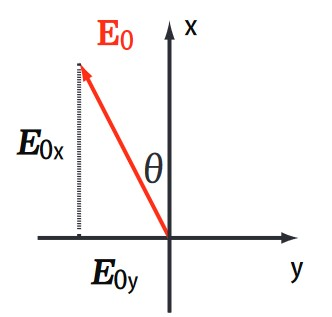
\includegraphics[width=0.3\textwidth]{linear_pol} \\
                 Линейная поляризация} &

    \makecell[c]{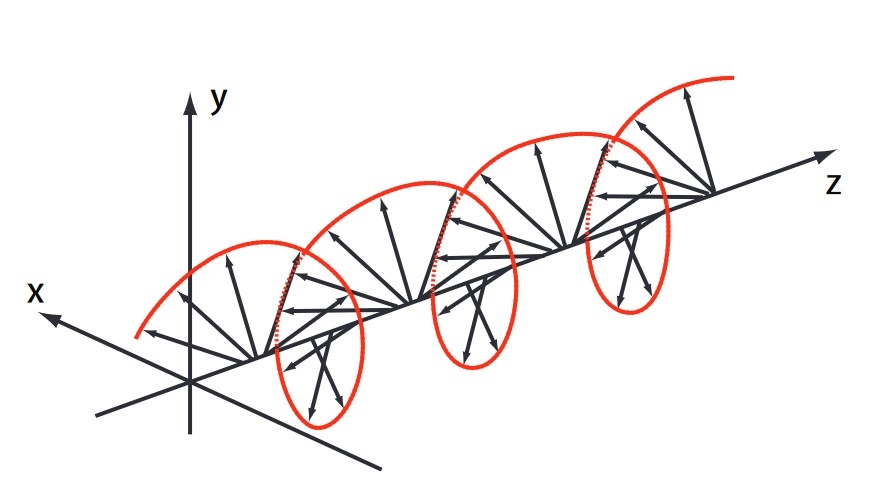
\includegraphics[width=0.3\textwidth]{circular_pol} \\
                 Круговая поляризация} \\
    \end{tabular}
}
\end{center}

}


\frame{
\frametitle{Закон Малюса}
\begin{columns}
    \column{0.6\textwidth} Поляризатор -- вещество, которое пропускает волны,
    колеблющиеся в одном выбранном направлении. Остальные же волны поглащаются.
    Соответсвенно, можно разложить исходное поле как на рисунке. Тогда после
    поляризатора получим волну с той же фазой, но амплитудой $E_1=E_0\cos\theta$.

    \column{0.4\textwidth} 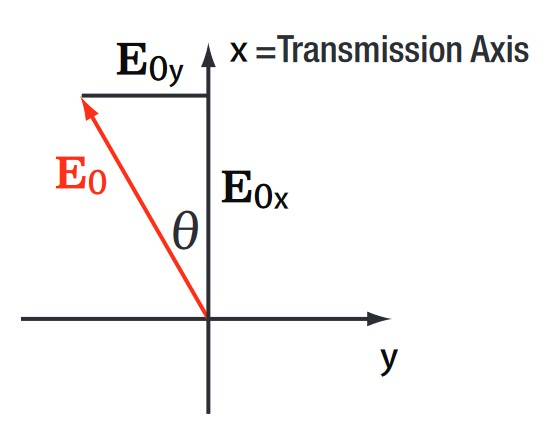
\includegraphics[width=\textwidth]{malus_polarizer.jpg}
\end{columns}

Отсюда для интенсивности получаем закон Малюса:
\[I = \langle E^2(t) \rangle \sim \cos^2\theta\]
}


\frame{
\begin{columns}
\column{0.6\textwidth}
В первом эксперименте (7.1.2) мы измеряли зависимость напряжения $U$ на фотодетекторе
от угла поляризатора $\theta$. Поскольку $U \sim I$, по закону Малюса ожидается,
что $U \sim \cos^2\theta$.

\column{0.4\textwidth}
    \begin{center}
        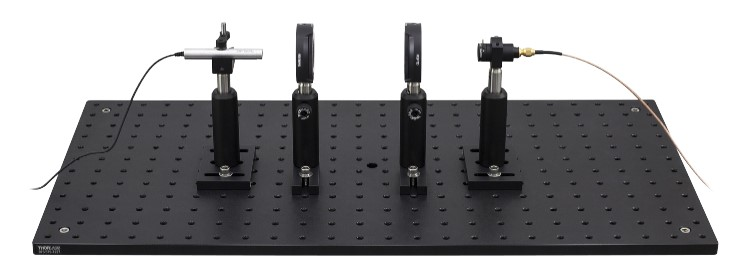
\includegraphics[width=\textwidth]{malus_ust1.jpg}
        Установка 7.1.2
    \end{center}
\end{columns}

\begin{center}
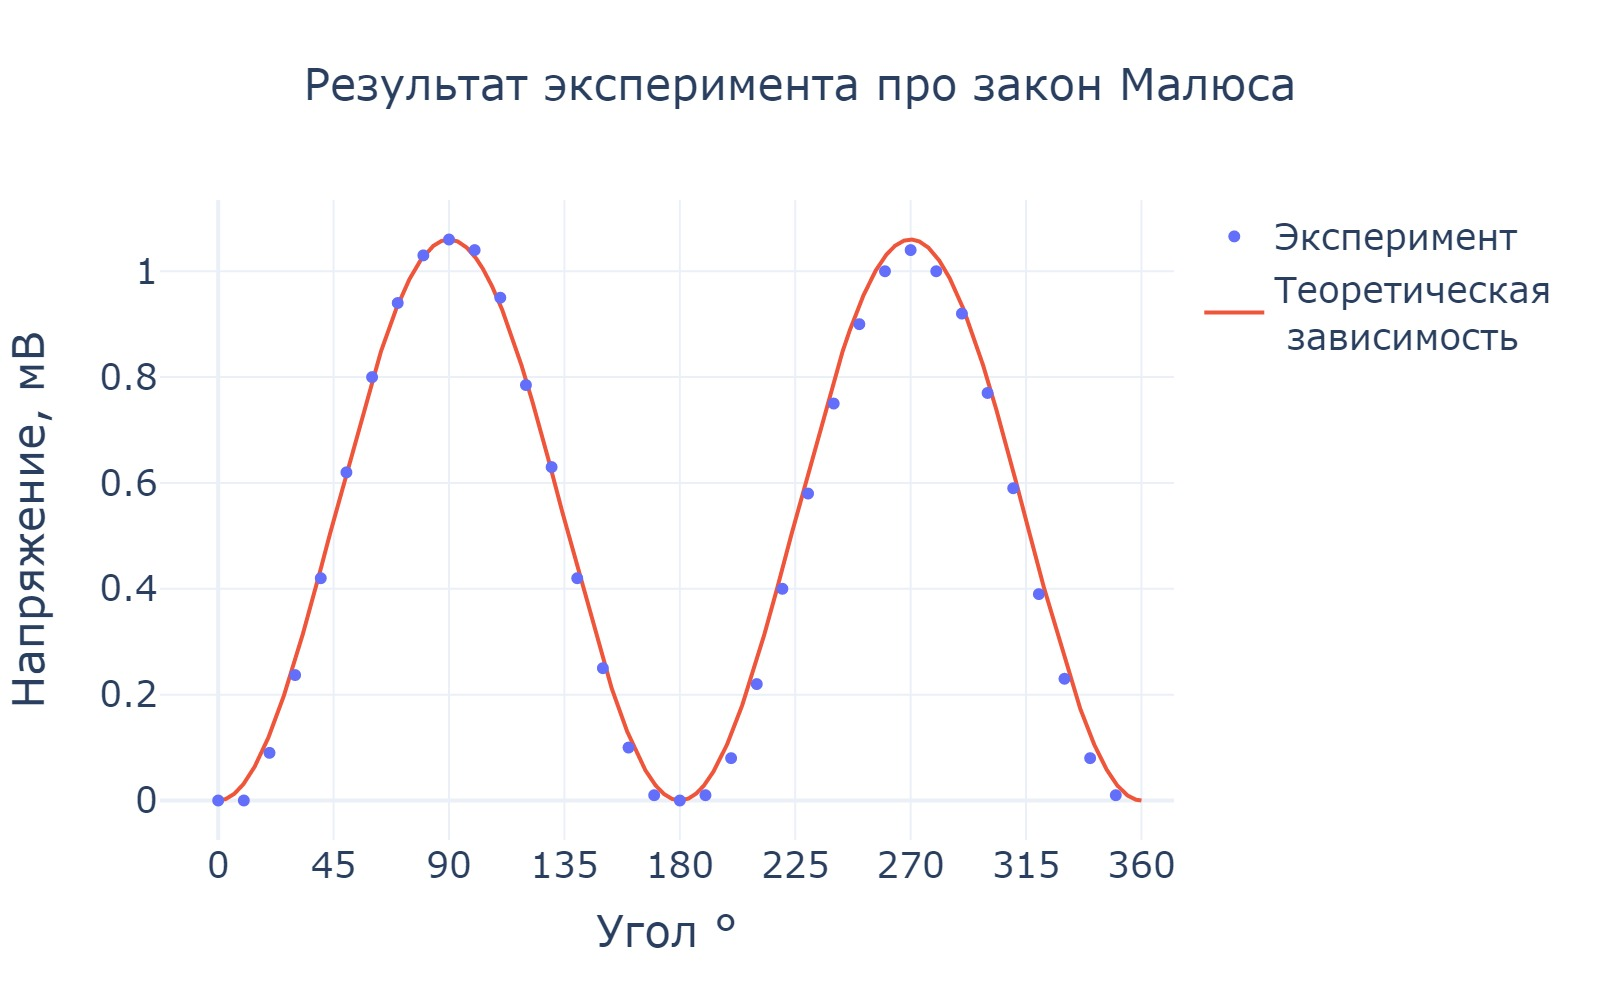
\includegraphics[scale=0.13]{712}
\end{center}
}


\frame{
\frametitle{Характер поляризации лазера}
\begin{columns}
    \column{0.6\textwidth}
    Расположим перед лазером поляризатор и измерим зависимость $U(\theta)$.
    Получим результат, соответствующий закону Малюса. $\Rightarrow$ лазер светит
    линейно поляризованным светом.

    \column{0.4\textwidth}
    \begin{center}
    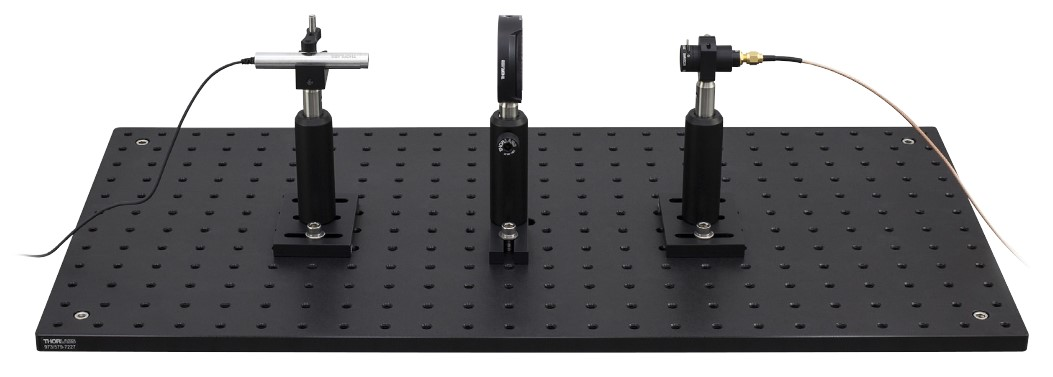
\includegraphics[width=\textwidth]{malus_ust2} \\
    Установка 7.1.3
    \end{center}
\end{columns}

\begin{center}
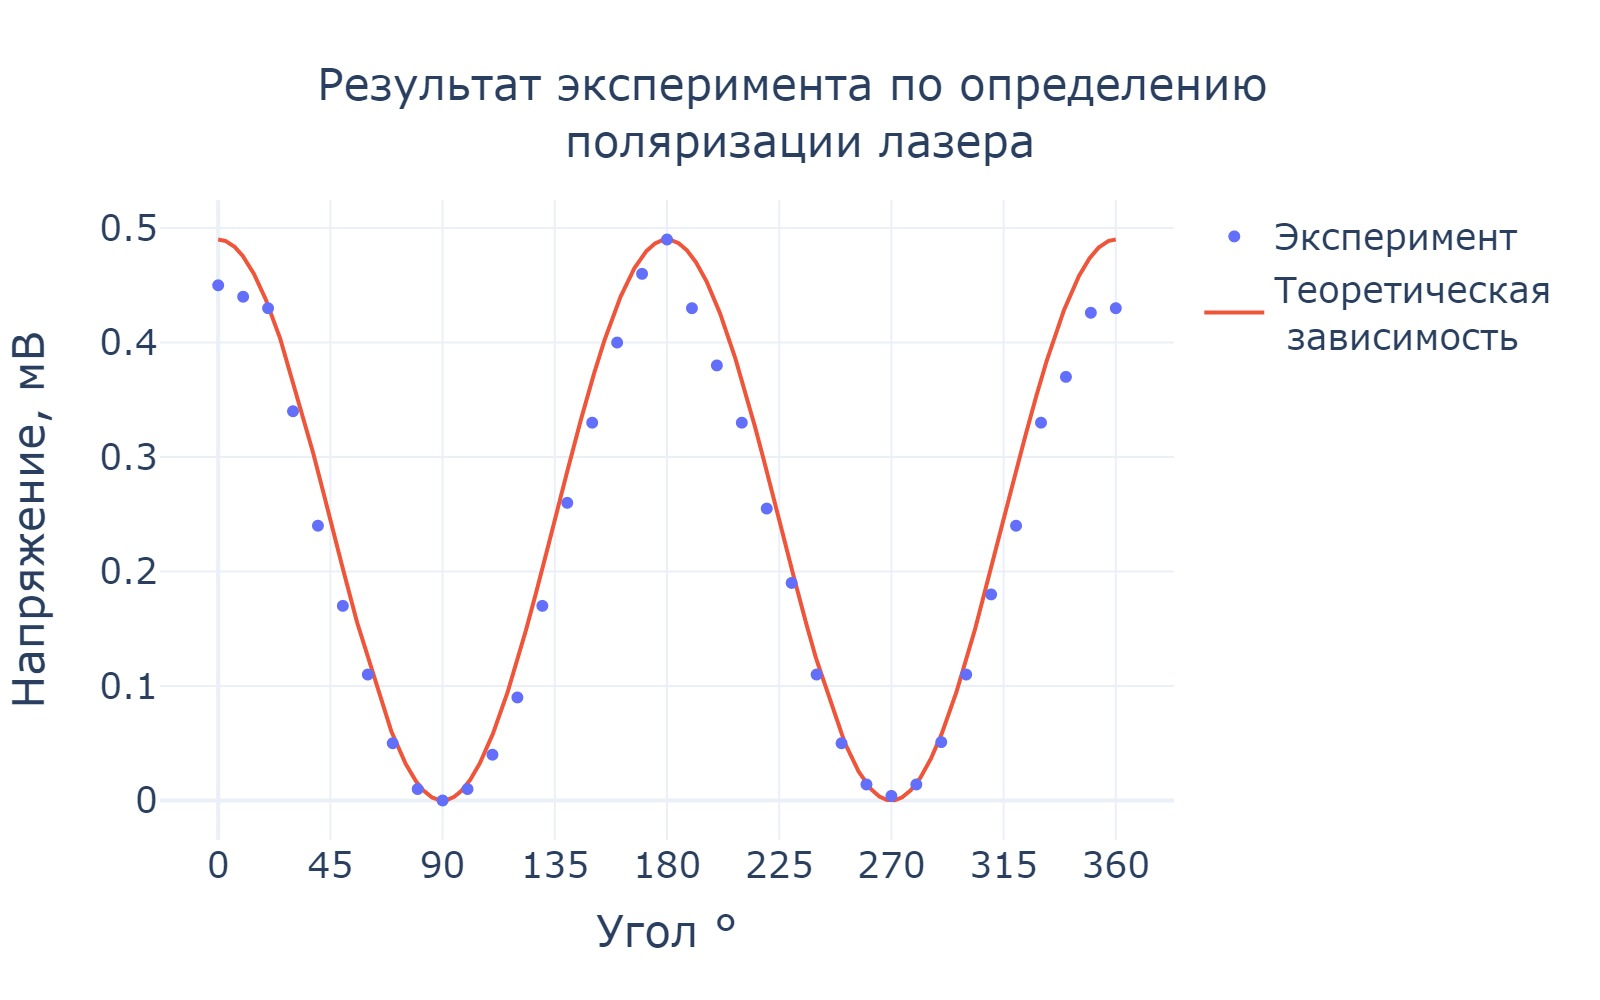
\includegraphics[scale=0.13]{713}
\end{center}
}


\frame{
\frametitle{Изучение пластинки $\lambda/4$}
Пластинка $\lambda/4$ имеет разные показатели преломления в зависимости от
направления падения волны. Т.к $v=c/n$, за время прохождения через пластинку между
компонентами $E_x$ и $E_y$ возникает разность фаз.
В случае круговой поляризации эта разность фаз равна должна быть равна $\pi/2$.

Если далее свет попадет на поляризатор, то его интенсивность не будет зависеть от
угла, под которым расположен этот поляризатор.


\begin{center}
    \makebox[\textwidth]{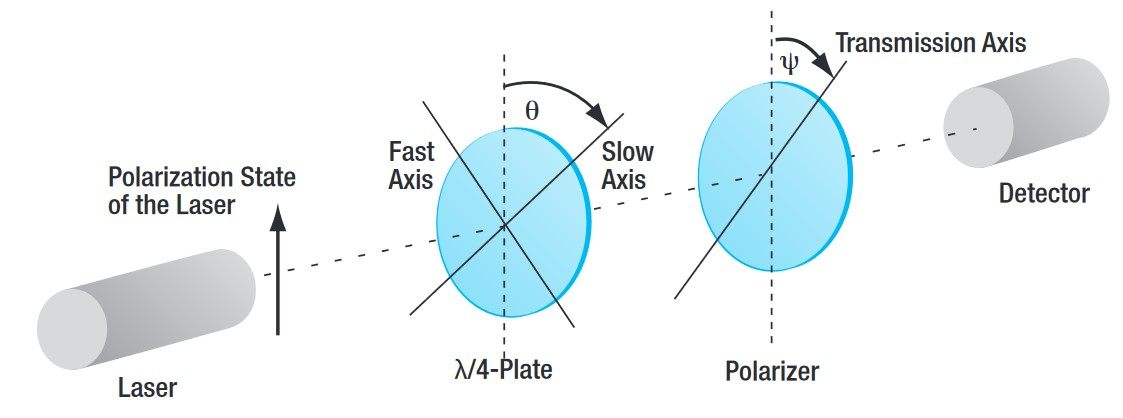
\includegraphics[scale=0.4]{quater_plate}}
\end{center}
}

\frame{
??? Получили расхождение с теорией.. мб что там пластинка плохая и поляризация
эллиптическая мб плохой вольтметр мб еще чтото хз

\begin{center}
    \makebox[\textwidth]{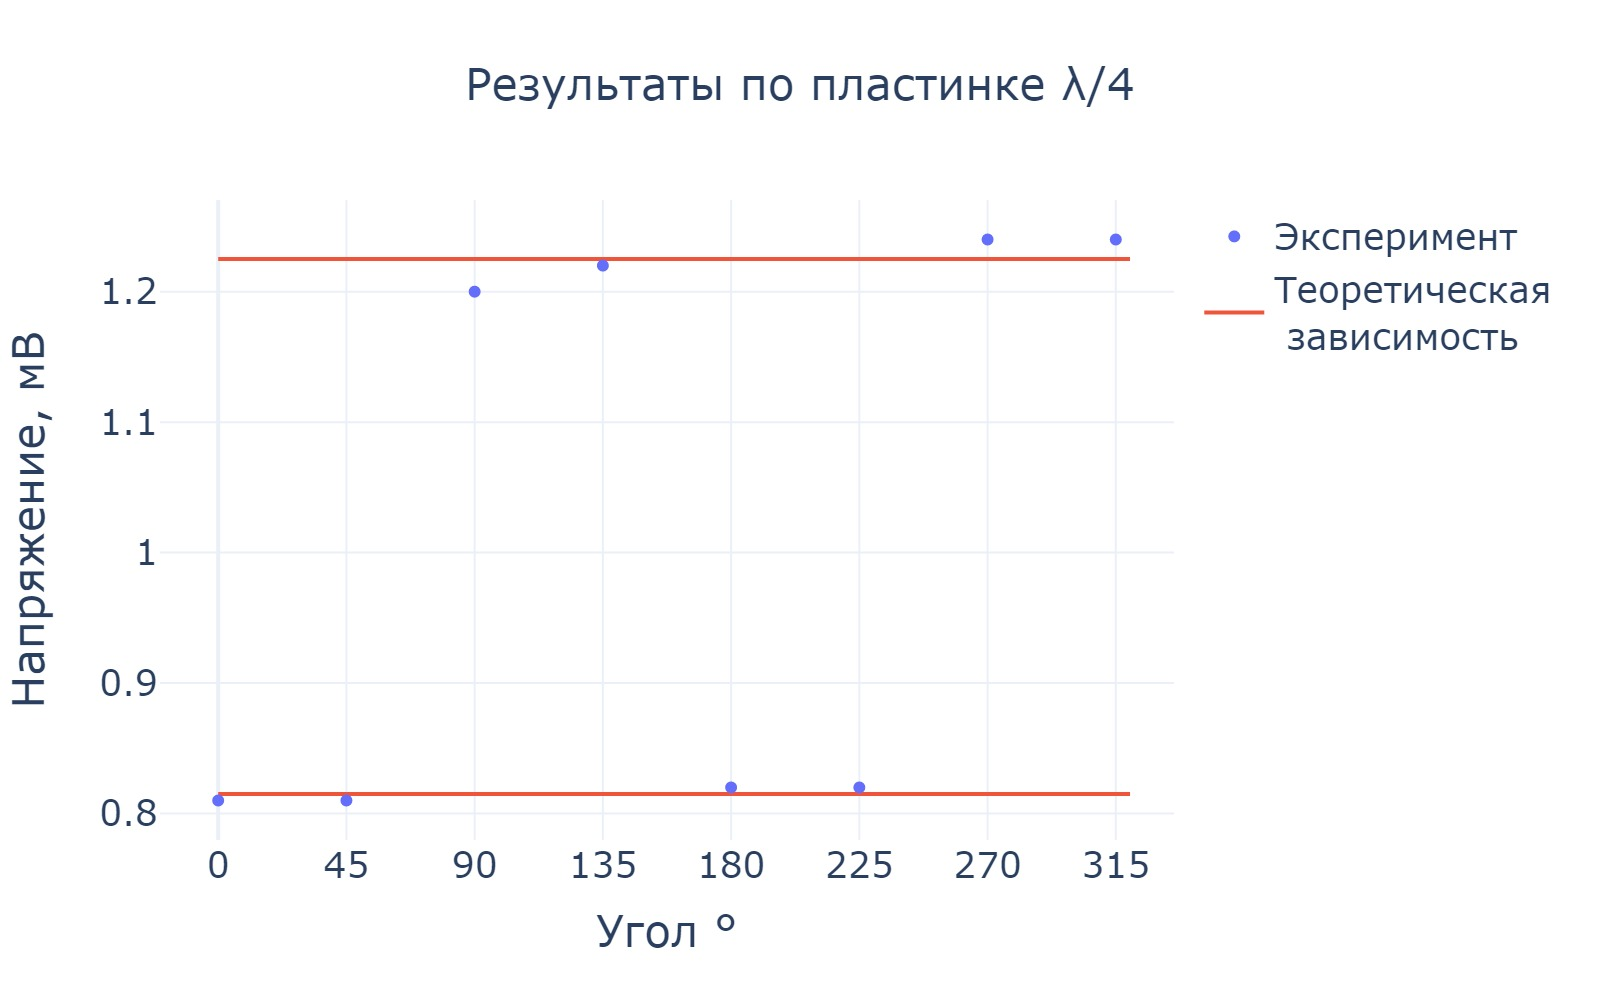
\includegraphics[width=0.7\textwidth]{715}}
\end{center}

}


%%%%%%%%%%%%%%%%%%%%%%%%%%%%%%%%% КОНЕЦ ПЕРВОЙ ЧАСТИ %%%%%%%%%%%%%%%%%%%%%%%%%%%%%%%%%



\end{document}